\subsection{Eksempel}
Gennemgangen af metoden er beskrevet for i detalje for hver del, men det kan være svært at få overblikket over metoden.
Af denne grund gives her et eksempel der tager en fra de rå data og hele vejen til det aggregerede resultat.
Eksemplet der følges kan ses i \cref{fig:totalbanjo}.
%intro godt at give et eksempel
%gennemgang af hvert led
%resultatet er at man har regnet ud der soves derfra og dertil
\begin{sidewaysfigure}
	\begin{minipage}{0.2\textwidth}
		\begin{subfigure}{\linewidth}
			\centering
			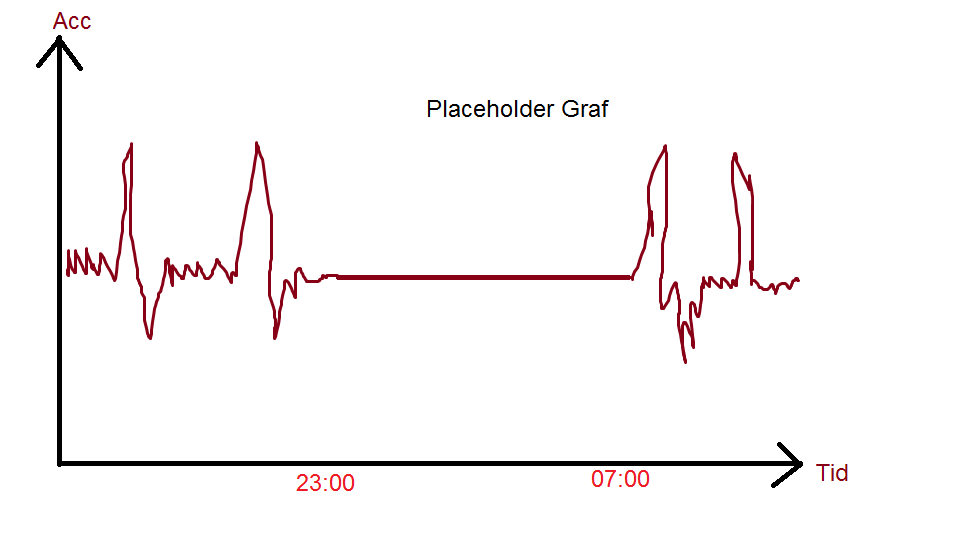
\includegraphics[scale=0.2]{acc-placeholder}
			\caption{Rå accelerations data.}\label{fig:rawaccplot}
		\end{subfigure}\\[5ex]
		\begin{subfigure}{\linewidth}
			\centering
			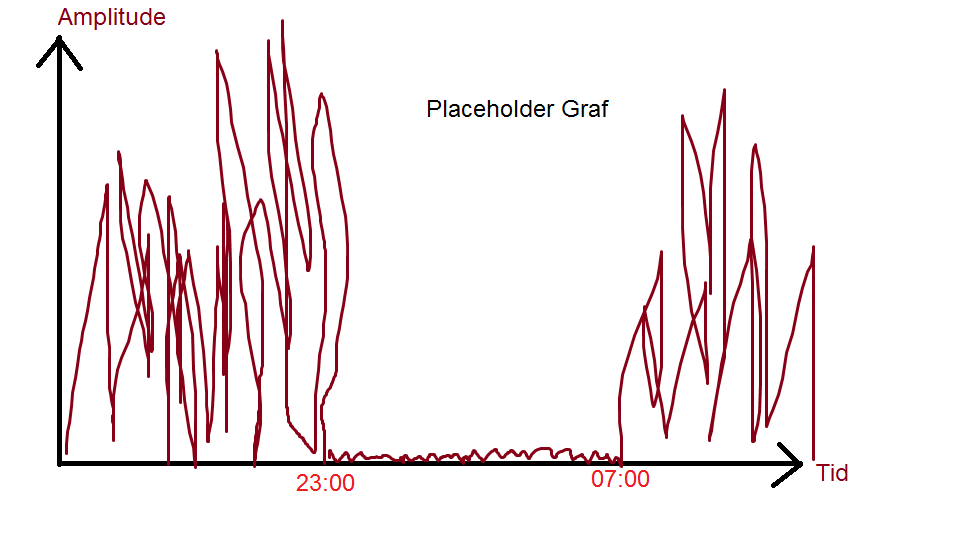
\includegraphics[scale=0.2]{ampl-placeholder}
			\caption{Rå amplitude data.}\label{fig:rawamplplot}
		\end{subfigure}
	\end{minipage}%
	\begin{minipage}{0.1\textwidth}
		\begin{subfigure}{\linewidth}
			\centering
			
\includegraphics[scale=0.3]{arrow}
		\end{subfigure}\\[15ex]
		\begin{subfigure}{\linewidth}
			\centering
			
\includegraphics[scale=0.3]{arrow}
		\end{subfigure}
	\end{minipage}%
	\begin{minipage}{0.2\textwidth}
		\begin{subfigure}{\linewidth}
			\centering
			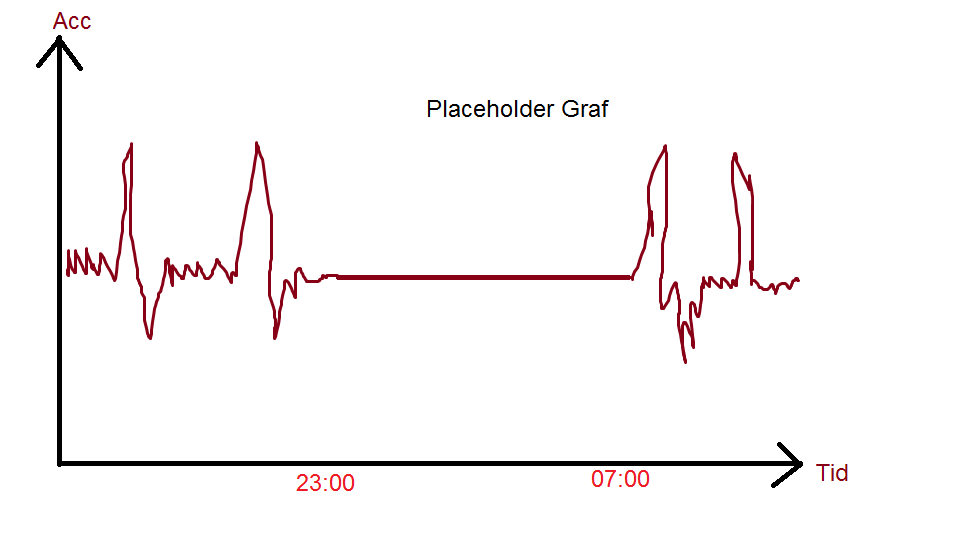
\includegraphics[scale=0.2]{acc-placeholder}
			\caption{Accelerations søvnestimering.}\label{fig:sleepcalcaccplot}
		\end{subfigure}\\[5ex]
		\begin{subfigure}{\linewidth}
			\centering
			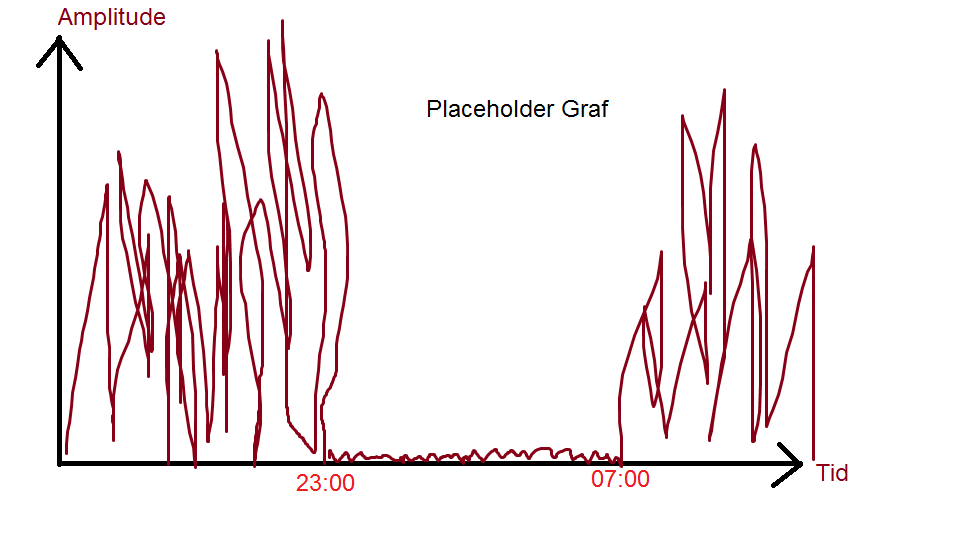
\includegraphics[scale=0.2]{ampl-placeholder}
			\caption{Amplitude søvnestimering}\label{fig:sleepcalcamplplot}
		\end{subfigure}
	\end{minipage}%
	\begin{minipage}{0.1\textwidth}
		\begin{subfigure}{\linewidth}
			\centering
			
\includegraphics[scale=0.2]{downarrow}
		\end{subfigure}\\[15ex]
		\begin{subfigure}{\linewidth}
			\centering
			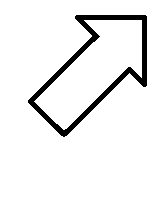
\includegraphics[scale=0.2]{uparrow}
		\end{subfigure}
	\end{minipage}%
	\begin{minipage}{0.2\textwidth}
		\begin{subfigure}{\linewidth}
			\centering
			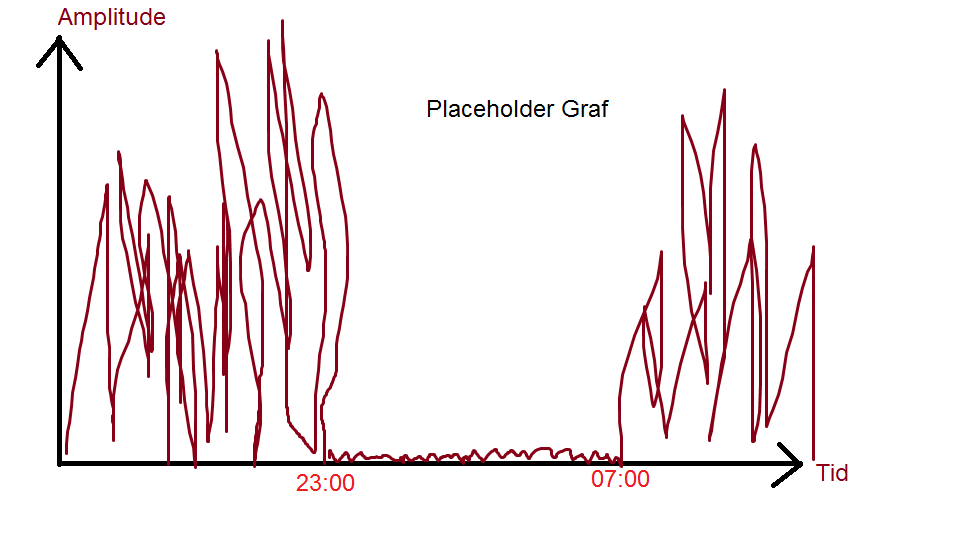
\includegraphics[scale=0.2]{ampl-placeholder}
			\caption{Kombineret søvnestimering}\label{fig:sleepcalcombine}
		\end{subfigure}
	\end{minipage}%
	\begin{minipage}{0.1\textwidth}
		\begin{subfigure}{\linewidth}
			\centering
			
\includegraphics[scale=0.3]{arrow}
		\end{subfigure}
	\end{minipage}%
	\begin{minipage}{0.07\textwidth}
		\begin{subfigure}{\linewidth}
			\centering
			\rotatebox{270}{\begin{tabular}{|c|c|c|}
			\hline starttid & sluttid & sandsynlighed \\ 
			\hline 20-20-2015 00:01 & 20-20-2015 08:05 & 0.99 \\ 
			\hline 
			\end{tabular}}
			\caption{Aggregering.}\label{fig:finalagg}
		\end{subfigure}
	\end{minipage}
	\caption{Illustration af søvnestimering fra rå data til aggregering.}\label{fig:totalbanjo}
\end{sidewaysfigure}

Der startes med de rå accelerations og amplitude data der kan ses i \cref{fig:rawaccplot} og \cref{fig:rawamplplot}.
På dette dataset foretages en række metoder beskrevet blablabla.